\chapter{Probability}
\label{probability}

\index{probability|(} 

What are the chances that a woman with an abnormal mammogram has breast cancer?  What is the likelihood that an overweight male teenager with high blood pressure will develop cardiovascular disease by the age of 50?  What is the probability that two parents who are unaffected carriers of a genetic mutation that causes cystic fibrosis will have a child that suffers from the disease. All of these questions use the language of probability, and despite how easy it is to ask these questions,  answers are not always easy to come by.  Probability also forms the foundation for data analysis and statistical inference, since nearly every conclusion to a study should be accompanied by a measure of uncertainty.  In the publication of  LEAP study discussed in Chapter 1, the manuscript included the probability that the results of the study could have been due simply to chance variation (a very small probability, as will be seen later in the text).

Like all mathematical tools, probability becomes easier to understand and work with when the important concepts and language have been formalized.   With the right tools, seemingly difficult problems can be solved in a series of reliable, reproducible steps.  This chapter introduces that formalization, using two types of examples.  One set of examples uses familiar terms using settings most people have seen before -- the outcomes of rolling dice or picking cards from a deck of playing cards.  The second type of examples are drawn from medicine, biology or public health, and reflect the context and language used in those fields. The approaches to solving both types of problems are surprisingly similar, once the problem has been posed clearly.

\section{Defining probability}
\label{basicsOfProbability}

\subsection{Some examples}

\textit{Some of these dice examples can be dropped, but leaving them for now in case they are reference later. }

We begin with some familiar examples.

\begin{example}\label{dieAllOutcomesex}{A ``die'', the singular of dice, is a cube with six faces numbered \resp{1}, \resp{2}, \resp{3}, \resp{4}, \resp{5}, and \resp{6}. What is the chance of getting \resp{1} when rolling a die?}\label{probOf1}
If the die is fair, then the chance of a \resp{1} is as good as the chance of any other number. Since there are six outcomes, the chance must be 1-in-6 or, equivalently, $1/6$.
\end{example}

\begin{example}{What is the chance of getting a \resp{1} or \resp{2} in the next roll?}\label{probOf1Or2}
\resp{1} and \resp{2} constitute two of the six equally likely possible outcomes, so the chance of getting one of these two outcomes must be $2/6 = 1/3$.
\end{example}

\begin{example}{What is the chance of getting either \resp{1}, \resp{2}, \resp{3}, \resp{4}, \resp{5}, or \resp{6} on the next roll?}\label{probOf123456}
100\%. The outcome must be one of these numbers.
\end{example}

\begin{example}{What is the chance of not rolling a \resp{2}?}\label{probNot2}
Since the chance of rolling a \resp{2} is $1/6$ or $16.\bar{6}\%$, the chance of not rolling a \resp{2} must be $100\% - 16.\bar{6}\%=83.\bar{3}\%$ or $5/6$.

Alternatively, we could have noticed that not rolling a \resp{2} is the same as getting a \resp{1}, \resp{3}, \resp{4}, \resp{5}, or \resp{6}, which makes up five of the six equally likely outcomes and has probability $5/6$.
\end{example}

\begin{example}\label{dieProportionProbex} {Consider rolling two dice. If $1/6^{th}$ of the time the first die is a \resp{1} and $1/6^{th}$ of those times the second die is a \resp{1}, what is the chance of getting two \resp{1}s?}\label{probOf2Ones}
If $16.\bar{6}$\% of the time the first die is a \resp{1} and $1/6^{th}$ of \emph{those} times the second die is also a \resp{1}, then the chance that both dice are \resp{1} is $(1/6)\times (1/6)$ or $1/36$.
\end{example}

Here is an example from genetics.

\begin{example}
Cystic fibrosis (CF) is a life-threatening genetic disorder characterized by the buildup of thick mucus in the lungs and pancreas, caused by mutations in the \textit{CFTR} gene located on chromosome 7. Defective copies of \textit{CFTR} can result in the reduced quantity and/or function of the CFTR protein, which transports sodium and chloride across cell membranes. CF is an autosomal recessive disorder -- an individual only develops CF if they have inherited two affected copies of \textit{CFTR}. Individuals with one normal (wild-type) copy and one defective (mutated) copy are known as carriers; they do not develop CF, but may pass the disease-causing mutation onto their offspring.

Suppose that both members of a couple are CF carriers. What is the probability that a child of this couple will be affected by CF?  The problem sounds a bit more complicated than calculating probabilities for the outcome of rolling a die, but can be solved with the same simple methods.  We show two solutions.

\textit{Solution 1: Enumerate all of the possible outcomes and exploit the fact that the outcomes are equally likely, as in \ref{dieAllOutcomesex}  During reproduction, each parent passes along one copy of the \textit{CFTR} gene, with each copy passed along with probability 1/2. Figure \ref{fig:cfInheritance} shows the four possible genotypes for a child of these parents, with the paternal chromosome in blue, the maternal chromosome in green,  chromosomes with the wild-type and mutated version of CFTR marked with $+$ and$-$.  Each of the four outcomes (wild-type CFTR, wild-type CFTR),  (wild-type CFTR, CFTR mutation) (CFTR mutation, wild-type CFTR) and (CFTR mutation, CFTR mutation), so the child will be affected with probability $1/4$.  It is important to recognize that the child being an unaffected carrier consists of two distinct outcomes, not one.

\textit{Solution 2:  Calculate the proportion of outcomes that produce an affected child, as in \ref{dieProportionProbex}.}  During reproduction, half of the time, the mother will pass along an affected gene.  When the child receives an affected gene from the mother, about half of those times, the father will have passed along an affected gene.	So the proportion of times the child will be affected is $(1/2) \times (1/2) = 1/4$.
\end{example}

\begin{figure}
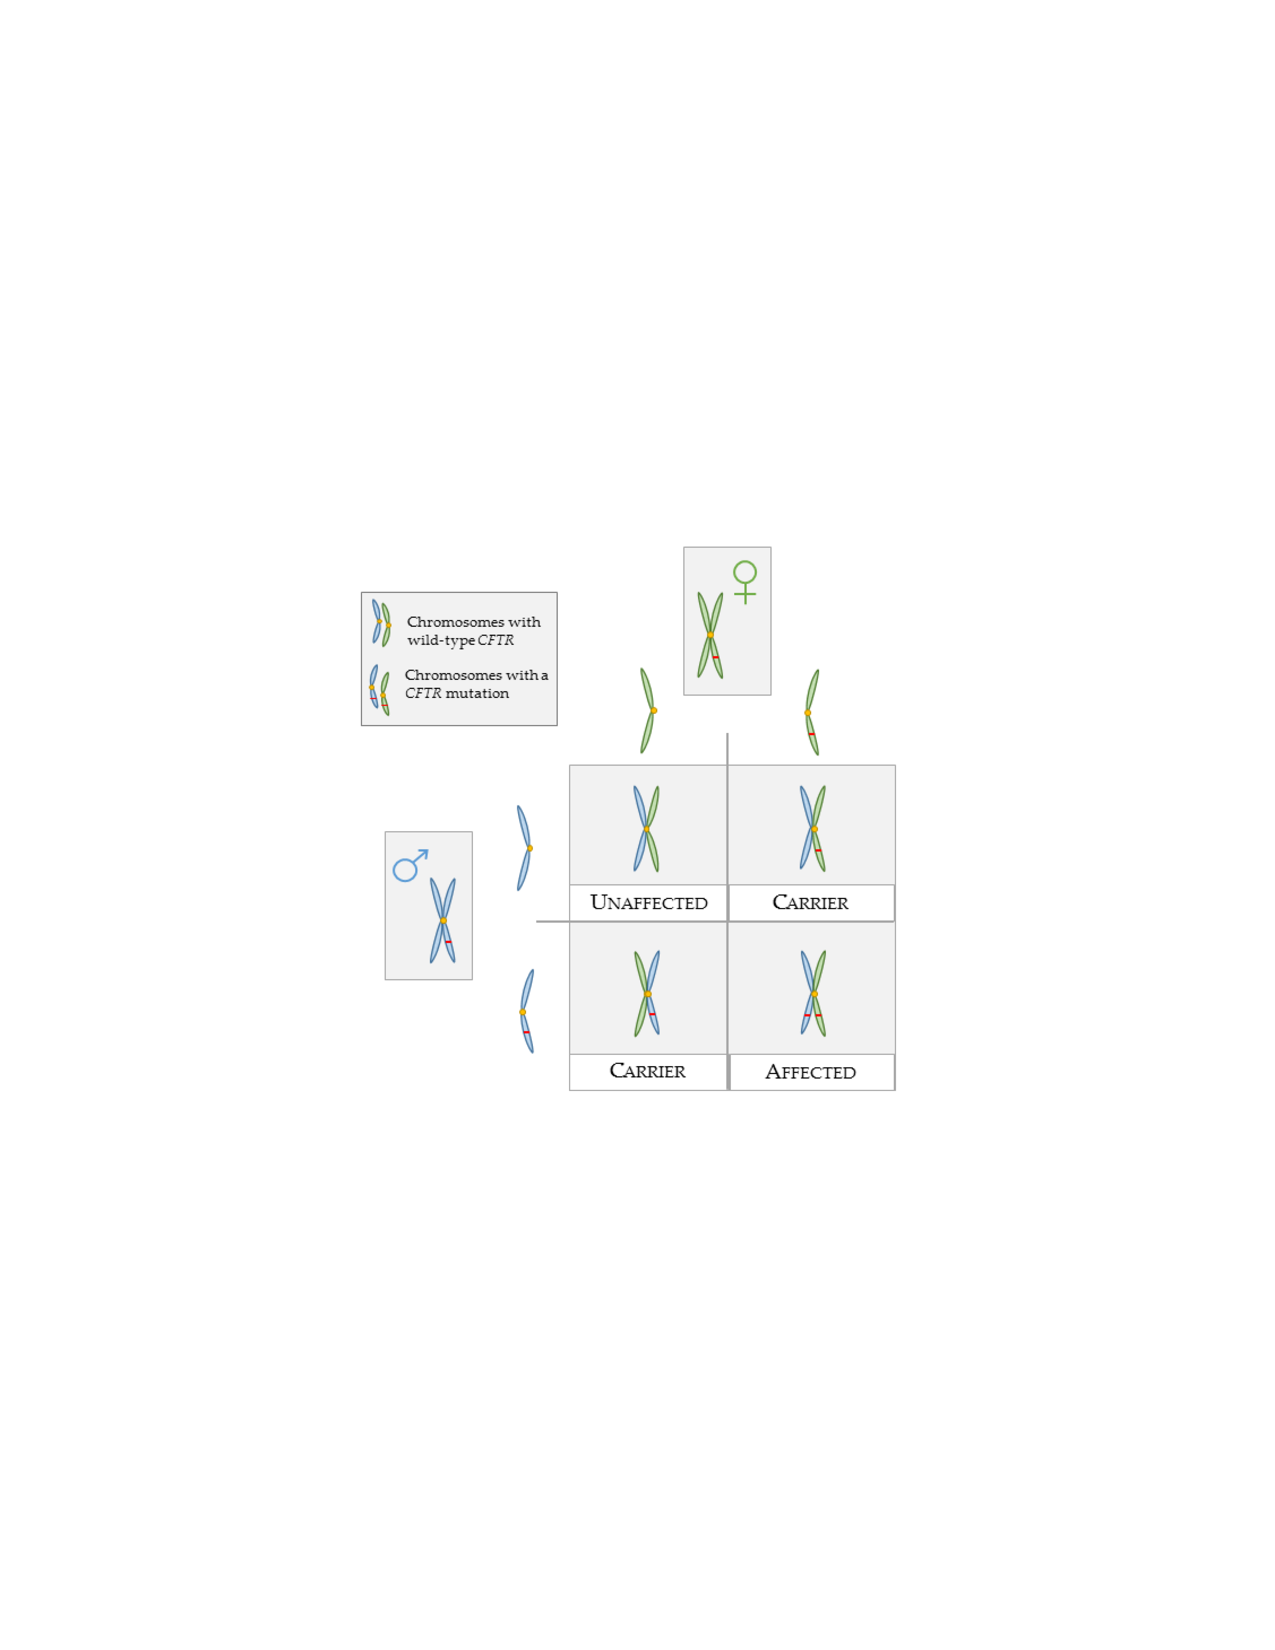
\includegraphics[width= 0.75\textwidth]{./figures/cfInheritance/cfInheritance.pdf}
\caption{Pattern of inheritance of a child of two unaffected carriers of CFTR}
\label{fig:cfInheritance}
\end{figure}


\begin{exercise}
Suppose the father is affected by CF and the mother is an unaffected carrier.  What is the probability that their child will be affected by the disease?

\textit{Solution}  Since the father is affected, he will always pass along a defective copy of the gene.  Since the mother will pass along a defective copy half of the time, the child will be affected half of the time, or with probability $1/4$.

\end{exercise}

\subsection{Probability}

\index{random phenomena |(}

Probability is used to assign a level of uncertainty to outcomes of phenomena that are happen randomly (rolling dice, passing along a defective gene during reproduction), or appear random because of a lack of understanding about exactly  how the phenomenon occurs (an obese teenager with high blood pressure developing cardiovascular disease later in life).In either case, the interpretation is the same -- the chance that some event will happen in the future -- and modeling these complex phenomena as random can be useful.

Mathematicians and philosophers have struggled for centuries (literally) to arrive at a clear statement of how probability is defined, or what it means.  In this text we use the most common definition, which also has the clearest interpretation.

\begin{termBox}{\tBoxTitle{Probability}
The \term{probability} of an outcome is the proportion of times the outcome would occur if the random phenomenon could be observed an infinite number of times.}
\end{termBox}

Probability is defined as a proportion, and it always takes values between 0~and~1 (inclusively). It may also be displayed as a percentage between 0\% and 100\%.

It is easy to imagine rolling dice a large number of times to observe the law of large numbers, but for examples like the CF example, the interpretation of probability is more hypothetical, since family sizes are typically small.  But it is not too difficult to imagine a thought experiment in which two parents have many children.  If the two parents are unaffected carriers, approximately 25\% of their off spring will suffer from CF.

This definition of probability can be illustrated by rolling a die many times. Let $\hat{p}_n$ be the proportion of outcomes that are \resp{1} after the first $n$ rolls. As the number of rolls increases, $\hat{p}_n$ will converge to the probability of rolling a \resp{1}, $p = 1/6$. Figure~\ref{dieProp} shows this convergence for 100,000 die rolls. The tendency of $\hat{p}_n$ to stabilize around $p$ is described by the \term{Law of Large Numbers}. 

\begin{figure}[bt]
\centering
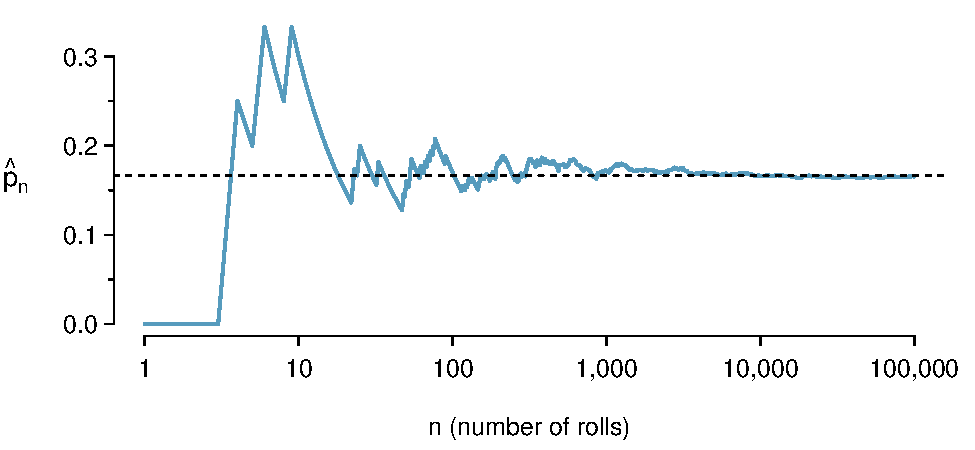
\includegraphics[width=0.85\textwidth]{ch_probability_oi_biostat/figures/dieProp/dieProp}
\caption{The fraction of die rolls that are 1 at each stage in a simulation. The proportion tends to get closer to the probability $1/6 \approx 0.167$ as the number of rolls increases.}
\label{fig:dieProp}
\end{figure}

The behavior shown in \ref{fig:dieProp} matches most people's intuition about probability, but proving mathematically that the behavior is always true is surprisingly difficult and is beyond the level of this text.  Mathematicians call the result \textit{The Law of Large Numbers}, which is used to justify mathematically this intuitively appealing definition.

\index{Law of Large Numbers |(}

\begin{termBox}{\tBoxTitle{Law of Large Numbers}
As more observations are collected, the proportion $\hat{p}_n$ of occurrences with a particular outcome converges to the probability $p$ of that outcome.}
\end{termBox}

Occasionally the proportion will veer off from the probability and appear to defy the Law of Large Numbers, as $\hat{p}_n$ does many times in Figure~\ref{dieProp}. However, these deviations become smaller as the number of rolls increases.

The notation $p$ is the probability of rolling a \resp{1}. We can also write this probability as
\begin{eqnarray*}
P(\text{rolling a \resp{1}})
\end{eqnarray*}
\marginpar[\raggedright\vspace{-13mm}

$P(A)$\vspace{1mm}\\\footnotesize Probability of\\outcome $A$]{\raggedright\vspace{-13mm}

$P(A)$\vspace{1mm}\\\footnotesize Probability of\\outcome $A$}As we become more comfortable with this notation, we will abbreviate it further. For instance, if it is clear that the process is ``rolling a die'', we could abbreviate $P($rolling a \resp{1}$)$ as~$P($\resp{1}$)$. 

\subsection{Disjoint or mutually exclusive outcomes}

\index{disjoint|(}
\index{mutually exclusive|(}

Two outcomes are called \term{disjoint} or \term{mutually exclusive} if they cannot both happen. When rolling a die, the outcomes \resp{1} and \resp{2} are disjoint since they cannot both occur.  In the cystic fibrosis example, the two outcomes of a wild-type gene from the mother and a mutated gene from the father and a mutated gene from the mother, wild-type from the father are disjoint.   In the die example, the outcomes \resp{1} and ``rolling an odd number'' are not disjoint since both occur if the outcome of the roll is a \resp{1}. The outcomes of a child being affected and having at least one mutated copy of CFTR and  not disjoint. The terms \emph{disjoint} and \emph{mutually exclusive} are equivalent and interchangeable.

Calculating the probability of disjoint outcomes is easy. When rolling a die, the outcomes \resp{1} and \resp{2} are disjoint, and we compute the probability that one of these outcomes will occur by adding their separate probabilities:
\begin{eqnarray*}
P(\text{\resp{1} or \resp{2}}) = P(\text{\resp{1}})+P(\text{\resp{2}}) = 1/6 + 1/6 = 1/3
\end{eqnarray*}
What about  the probability of rolling a \resp{1}, \resp{2}, \resp{3}, \resp{4}, \resp{5}, or \resp{6}? Here again, all of the outcomes are disjoint so we add the probabilities:
\begin{eqnarray*}
&&P(\text{\resp{1} or \resp{2} or \resp{3} or \resp{4} or \resp{5} or \resp{6}}) \\
	&&\quad= P(\text{\resp{1}})+P(\text{\resp{2}})+P(\text{\resp{3}})+P(\text{\resp{4}})+P(\text{\resp{5}})+P(\text{\resp{6}}) \\
	&&\quad= 1/6 + 1/6 + 1/6 + 1/6 + 1/6 + 1/6 = 1.
\end{eqnarray*}
The probability that a child will be an unaffected carrier in the CF example is $(1/2) = (1/2) = 1/4$.

The \term{Addition Rule} guarantees the accuracy of this approach when the outcomes are disjoint. 

\begin{termBox}{\tBoxTitle{Addition Rule of disjoint outcomes} If $A_1$ and $A_2$ represent two disjoint outcomes, then the probability that one of them occurs is given by
\begin{eqnarray*}
P(A_1\text{ or } A_2) = P(A_1) + P(A_2)
\end{eqnarray*}
If there are many disjoint outcomes $A_1$, ..., $A_k$, then the probability that one of these outcomes will occur is
\begin{eqnarray}
P(A_1) + P(A_2) + \cdots + P(A_k)
\end{eqnarray}
}
\end{termBox}

Probability problems rarely consider individual outcomes and instead consider \indexthis{\emph{sets}}{sets} or \indexthis{\emph{collections}}{collections} of outcomes. Let $A$ represent the event where a die roll results in \resp{1} or \resp{2} and $B$~represent the event that the die roll is a \resp{4} or a \resp{6}. We write $A$ as the set of outcomes $\{$\resp{1},~\resp{2}$\}$ and $B=\{$\resp{4}, \resp{6}$\}$. These sets are commonly called \termsub{events}{event}. Because $A$ and $B$ have no elements in common, they are disjoint events. $A$ and $B$ are represented in Figure~\ref{disjointSets}.

\begin{figure}[hhh]
\centering
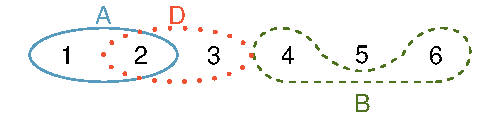
\includegraphics[width=0.55\textwidth]{ch_probability/figures/disjointSets/disjointSets}
\caption{Three events, $A$, $B$, and $D$, consist of outcomes from rolling a die. $A$ and $B$ are disjoint since they do not have any outcomes in common.}
\label{disjointSets}
\end{figure}

The Addition Rule applies to both disjoint outcomes and disjoint events. The probability that one of the disjoint events $A$ or $B$ occurs is the sum of the separate probabilities:
\begin{align*}
P(A\text{ or }B) = P(A) + P(B) = 1/3 + 1/3 = 2/3
\end{align*}

\begin{exercise}
(a) Verify the probability of event $A$, $P(A)$, is $1/3$ using the Addition Rule. (b) Do the same for event $B$.\footnote{(a) $P(A) = P($\resp{1} or \resp{2}$) = P($\resp{1}$) + P($\resp{2}$) = \frac{1}{6} + \frac{1}{6} = \frac{2}{6} = \frac{1}{3}$. (b) Similarly, $P(B) = 1/3$.}
\end{exercise}

\begin{exercise} \label{exerExaminingDisjointSetsABD}
(a) Using Figure~\ref{disjointSets} as a reference, what outcomes are represented by event $D$? (b) Are events $B$ and $D$ disjoint? (c) Are events $A$ and $D$ disjoint?\footnote{(a)~Outcomes \resp{2} and \resp{3}. (b)~Yes, events $B$ and $D$ are disjoint because they share no outcomes. (c)~The events $A$ and $D$ share an outcome in common, \resp{2}, and so are not disjoint.}
\end{exercise}

\begin{exercise}
In Guided Practice~\ref{exerExaminingDisjointSetsABD}, you confirmed $B$ and $D$ from Figure~\ref{disjointSets} are disjoint. Compute the probability that event $B$ or event $D$~occurs.\footnote{Since $B$ and $D$ are disjoint events, use the Addition Rule: $P(B$ or $D) = P(B) + P(D) = \frac{1}{3} + \frac{1}{3} = \frac{2}{3}$.}
\end{exercise}

\textit{should we add more genetics problems here?  I have removed the email example because of the possible confusion between events involving sampling from a population vs a study sample.  If we think we can make that clear, we can use examples from famuss, perhaps by posing a problem of sampling members from the study participants.  Note also that this is moving more slowly than the Stat 102 notes, but we did show some of this material on the blackboard.  If we use this chapter in 102, perhaps we can move quickly to more complicated examples.}

\index{event|)}
\index{disjoint|)}
\index{mutually exclusive|)}

\subsection{Probabilities when events are not disjoint}

Let's consider calculations for two events that are not disjoint in the context of a \indexthis{regular deck of 52 cards}{deck of cards}, represented in Table~\ref{deckOfCards}. If you are unfamiliar with the cards in a regular deck, please see the footnote.\footnote{The 52 cards are split into four \term{suits}: $\clubsuit$ (club), {\color{redcards}$\diamondsuit$} (diamond), {\color{redcards}$\heartsuit$} (heart), $\spadesuit$ (spade). Each suit has its 13 cards labeled: \resp{2}, \resp{3}, ..., \resp{10}, \resp{J} (jack), \resp{Q} (queen), \resp{K} (king), and \resp{A} (ace). Thus, each card is a unique combination of a suit and a label, e.g. {\color{redcards}\resp{4$\heartsuit$}} and \resp{J$\clubsuit$}. The 12 cards represented by the jacks, queens, and kings are called \termsub{\resp{face cards}}{face card}. The cards that are {\color{redcards}$\diamondsuit$} or {\color{redcards}$\heartsuit$} are typically colored {\color{redcards}red} while the other two suits are typically colored black.}

\begin{table}[h]
\centering
\begin{tabular}{lll lll lll lll l}
\resp{2$\clubsuit$} & \resp{3$\clubsuit$} & \resp{4$\clubsuit$} & \resp{5$\clubsuit$} & \resp{6$\clubsuit$} & \resp{7$\clubsuit$} & \resp{8$\clubsuit$} & \resp{9$\clubsuit$} & \resp{10$\clubsuit$} & \resp{J$\clubsuit$} & \resp{Q$\clubsuit$} & \resp{K$\clubsuit$} & \resp{A$\clubsuit$}  \\
\color{redcards} \resp{2$\diamondsuit$} & \color{redcards}\resp{3$\diamondsuit$} & \color{redcards}\resp{4$\diamondsuit$} & \color{redcards}\resp{5$\diamondsuit$} & \color{redcards}\resp{6$\diamondsuit$} & \color{redcards}\resp{7$\diamondsuit$} & \color{redcards}\resp{8$\diamondsuit$} & \color{redcards}\resp{9$\diamondsuit$} & \color{redcards}\resp{10$\diamondsuit$} & \color{redcards}\resp{J$\diamondsuit$} & \color{redcards}\resp{Q$\diamondsuit$} & \color{redcards}\resp{K$\diamondsuit$} & \color{redcards}\resp{A$\diamondsuit$} \\
\color{redcards}\resp{2$\heartsuit$} & \color{redcards}\resp{3$\heartsuit$} & \color{redcards}\resp{4$\heartsuit$} & \color{redcards}\resp{5$\heartsuit$} & \color{redcards}\resp{6$\heartsuit$} & \color{redcards}\resp{7$\heartsuit$} & \color{redcards}\resp{8$\heartsuit$} & \color{redcards}\resp{9$\heartsuit$} & \color{redcards}\resp{10$\heartsuit$} & \color{redcards}\resp{J$\heartsuit$} & \color{redcards}\resp{Q$\heartsuit$} & \color{redcards}\resp{K$\heartsuit$} & \color{redcards}\resp{A$\heartsuit$} \\
\resp{2$\spadesuit$} & \resp{3$\spadesuit$} & \resp{4$\spadesuit$} & \resp{5$\spadesuit$} & \resp{6$\spadesuit$} & \resp{7$\spadesuit$} & \resp{8$\spadesuit$} & \resp{9$\spadesuit$} & \resp{10$\spadesuit$} & \resp{J$\spadesuit$} & \resp{Q$\spadesuit$} & \resp{K$\spadesuit$} & \resp{A$\spadesuit$}
\end{tabular}
\caption{Representations of the 52 unique cards in a deck.}
\label{deckOfCards}
\end{table}

\begin{exercise}
(a) What is the probability that a randomly selected card is a diamond? (b)~What is the probability that a randomly selected card is a face card?\footnote{(a) There are 52 cards and 13 diamonds. If the cards are thoroughly shuffled, each card has an equal chance of being drawn, so the probability that a randomly selected card is a diamond is $P({\color{redcards}\diamondsuit}) = \frac{13}{52} = 0.250$. (b)~Likewise, there are 12 face cards, so $P($face card$) = \frac{12}{52} = \frac{3}{13} = 0.231$.}
\end{exercise}

\term{Venn diagrams} are useful when outcomes can be categorized as ``in'' or ``out'' for two or three variables, attributes, or random processes. The Venn diagram in Figure~\ref{cardsDiamondFaceVenn} uses a circle to represent diamonds and another to represent face cards. If a card is both a diamond and a face card, it falls into the intersection of the circles. If it is a diamond but not a face card, it will be in part of the left circle that is not in the right circle (and so on). The total number of cards that are diamonds is given by the total number of cards in the diamonds circle: $10+3=13$. The probabilities are also shown (e.g. $10/52 = 0.1923$).

\begin{figure}
\centering
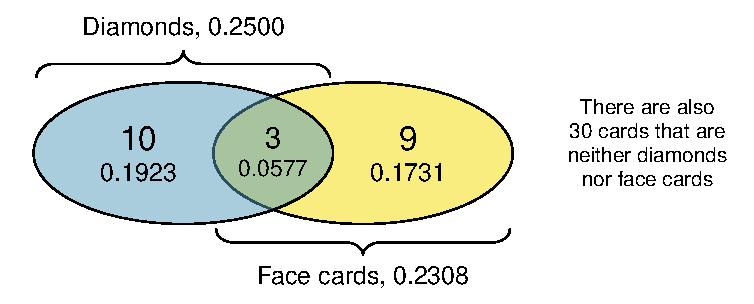
\includegraphics[width=0.65\textwidth]{ch_probability/figures/cardsDiamondFaceVenn/cardsDiamondFaceVenn}
\caption{A Venn diagram for diamonds and face cards.}
\label{cardsDiamondFaceVenn}
\end{figure}

%\begin{exercise}
%Using Figure~\ref{cardsDiamondFaceVenn}, verify $P($face card$) = 12/52=3/13$.\footnote{The Venn diagram shows face cards split up into ``face card but not {\color{redcards}$\diamondsuit$}'' and ``face card and {\color{redcards}$\diamondsuit$}''. Since these correspond to disjoint events, $P($face card$)$ is found by adding the two corresponding probabilities: $\frac{3}{52} + \frac{9}{52} = \frac{12}{52} = \frac{3}{13}$.}
%\end{exercise}

Let $A$ represent the event that a randomly selected card is a diamond and $B$ represent the event that it is a face card. How do we compute $P(A$ or $B)$? Events $A$ and $B$ are not disjoint -- the cards {\color{redcards}$J\diamondsuit$}, {\color{redcards}$Q\diamondsuit$}, and {\color{redcards}$K\diamondsuit$} fall into both categories -- so we cannot use the Addition Rule for disjoint events. Instead we use the Venn diagram. We start by adding the probabilities of the two events:
\begin{eqnarray*}
P(A) + P(B) = P({\color{redcards}\diamondsuit}) + P(\text{face card}) = 12/52 + 13/52
\label{overCountFaceDiamond}
\end{eqnarray*}
However, the three cards that are in both events were counted twice, once in each probability. We must correct this double counting:
\begin{eqnarray}
P(A\text{ or } B) &=&P(\text{face card or }{\color{redcards}\diamondsuit})  \notag \\
 &=& P(\text{face card}) + P({\color{redcards}\diamondsuit}) - P(\text{face card and }{\color{redcards}\diamondsuit}) \label{diamondFace} \\
 &=& 13/52 + 12/52 - 3/52 \notag \\
 &=& 22/52 = 11/26 \notag
\end{eqnarray}
Equation~(\ref{diamondFace}) is an example of the \term{General Addition Rule}. 

\begin{termBox}{\tBoxTitle{General Addition Rule} If $A$ and $B$ are any two events, disjoint or not, then the probability that at least one of them will occur is
\begin{eqnarray}
P(A\text{ or }B) = P(A) + P(B) - P(A\text{ and }B)
\label{generalAdditionRule}
\end{eqnarray}
where $P(A$ and $B)$ is the probability that both events occur.}
\end{termBox}

\begin{tipBox}{\tipBoxTitle{``or'' is inclusive}
When we write ``or'' in statistics, we mean ``and/or'' unless we explicitly state otherwise. Thus, $A$ or $B$ occurs means $A$, $B$, or both $A$ and $B$ occur.}
\end{tipBox}

\begin{exercise}
(a) If $A$ and $B$ are disjoint, describe why this implies $P(A$ and $B) = 0$. (b) Using part (a), verify that the General Addition Rule simplifies to the simpler Addition Rule for disjoint events if $A$ and $B$ are disjoint.\footnote{(a) If $A$ and $B$ are disjoint, $A$ and $B$ can never occur simultaneously. (b) If $A$ and $B$ are disjoint, then the last term of Equation~(\ref{generalAdditionRule}) is 0 (see part (a)) and we are left with the Addition Rule for disjoint events.}
\end{exercise}








